\section{The Derivative}

\subsection{The Limit Definition}

\begin{multicols}{2}

Recall that a \textbf{secant line} is a line between two points on the graph of a function. If $f$ is a function and $(a,f(a))$ and $(b,f(b))$ are \textit{different} points on the function, then the secant line that they determine has equation
$$y=f(a) + \frac{f(b)-f(a)}{b-a}(x-a).$$
We can assume $b>a$ and write $b=a+h$ for some $h>0$. Then the equation for the secant line through $(a,f(a))$ and $(b,f(b))=(a+h,f(a+h))$ is
$$y=f(a) + \frac{f(a+h)-f(a)}{h}(x-a).$$


Now we're going to use \textit{limits} to move one point $(b,f(b))$ closer to the other $(a,f(a))$, and see what happens to the secant line. Since the secant line passes through the point $(a,f(a))$, we only have to track what happens to the slope. As $b$ moves to $a$, the value of $h$ goes to $0$, so the slope of the secant line approaches
$$\lim_{h\to 0}\frac{f(a+h)-f(a)}{h}.$$
We'll denote this quantity $f'(a)$, and call this the \textbf{derivative of $f$ at $a$} (if this limit exists). The line through the point $(a,f(a))$ with slope $f'(a)$ is called the \textbf{tangent line of $f$ at $a$} and has equation
$$y=f(a)+f'(a)(x-a).$$

\columnbreak

\resizebox{3.25in}{!}{

\tikzset{every picture/.style={line width=0.75pt}}

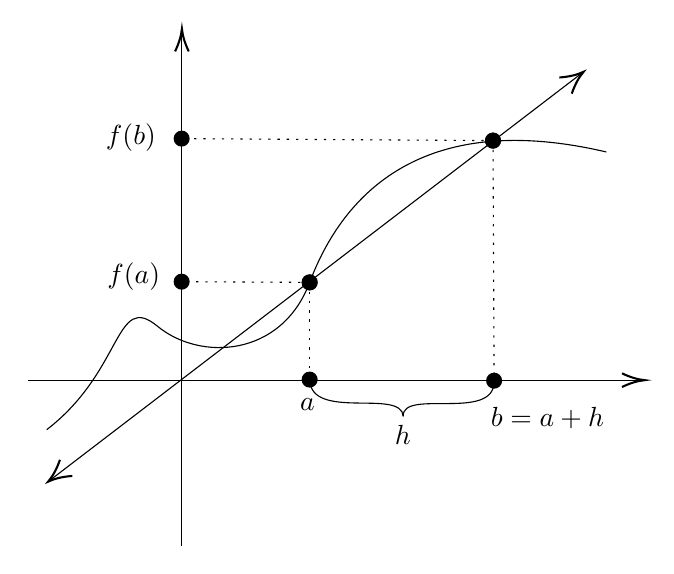
\begin{tikzpicture}[x=0.75pt,y=0.75pt,yscale=-1,xscale=1]
%uncomment if require: \path (0,441); %set diagram left start at 0, and has height of 441

%Straight Lines [id:da16102953695521127]
\draw    (163,221.33) -- (458,221.33) ;
\draw [shift={(460,221.33)}, rotate = 180] [color={rgb, 255:red, 0; green, 0; blue, 0 }  ][line width=0.75]    (10.93,-3.29) .. controls (6.95,-1.4) and (3.31,-0.3) .. (0,0) .. controls (3.31,0.3) and (6.95,1.4) .. (10.93,3.29)   ;
%Straight Lines [id:da9043079513680581]
\draw    (237.04,301) -- (237.04,54) ;
\draw [shift={(237.04,52)}, rotate = 90] [color={rgb, 255:red, 0; green, 0; blue, 0 }  ][line width=0.75]    (10.93,-3.29) .. controls (6.95,-1.4) and (3.31,-0.3) .. (0,0) .. controls (3.31,0.3) and (6.95,1.4) .. (10.93,3.29)   ;
%Curve Lines [id:da7565789477512073]
\draw    (171.9,245.19) .. controls (209.02,216.63) and (204.74,178.41) .. (225.27,195.34) .. controls (245.8,212.28) and (284.99,210.33) .. (298.59,174.22) .. controls (312.18,138.1) and (347.09,89.21) .. (441.52,111.39) ;
%Straight Lines [id:da9796385406474812]
\draw    (428.99,73.97) -- (174.17,269.02) ;
\draw [shift={(172.58,270.23)}, rotate = 322.57] [color={rgb, 255:red, 0; green, 0; blue, 0 }  ][line width=0.75]    (10.93,-4.9) .. controls (6.95,-2.3) and (3.31,-0.67) .. (0,0) .. controls (3.31,0.67) and (6.95,2.3) .. (10.93,4.9)   ;
\draw [shift={(430.57,72.75)}, rotate = 142.57] [color={rgb, 255:red, 0; green, 0; blue, 0 }  ][line width=0.75]    (10.93,-4.9) .. controls (6.95,-2.3) and (3.31,-0.67) .. (0,0) .. controls (3.31,0.67) and (6.95,2.3) .. (10.93,4.9)   ;
%Straight Lines [id:da4030910320179846]
\draw  [dash pattern={on 0.84pt off 2.51pt}]  (298.59,174.22) -- (298.59,221.05) ;
\draw [shift={(298.59,221.05)}, rotate = 90] [color={rgb, 255:red, 0; green, 0; blue, 0 }  ][fill={rgb, 255:red, 0; green, 0; blue, 0 }  ][line width=0.75]      (0, 0) circle [x radius= 3.35, y radius= 3.35]   ;
\draw [shift={(298.59,174.22)}, rotate = 90] [color={rgb, 255:red, 0; green, 0; blue, 0 }  ][fill={rgb, 255:red, 0; green, 0; blue, 0 }  ][line width=0.75]      (0, 0) circle [x radius= 3.35, y radius= 3.35]   ;
%Straight Lines [id:da14103701021608472]
\draw  [dash pattern={on 0.84pt off 2.51pt}]  (386.93,105.91) -- (387.46,221.58) ;
\draw [shift={(387.46,221.58)}, rotate = 89.74] [color={rgb, 255:red, 0; green, 0; blue, 0 }  ][fill={rgb, 255:red, 0; green, 0; blue, 0 }  ][line width=0.75]      (0, 0) circle [x radius= 3.35, y radius= 3.35]   ;
\draw [shift={(386.93,105.91)}, rotate = 89.74] [color={rgb, 255:red, 0; green, 0; blue, 0 }  ][fill={rgb, 255:red, 0; green, 0; blue, 0 }  ][line width=0.75]      (0, 0) circle [x radius= 3.35, y radius= 3.35]   ;
%Curve Lines [id:da47143485860977985]
\draw    (298.59,221.05) .. controls (299.18,241.14) and (342.98,225.16) .. (343.66,238.75) ;
%Curve Lines [id:da42610723931770456]
\draw    (387.46,221.58) .. controls (388.06,241.67) and (342.98,225.16) .. (343.66,238.75) ;
%Straight Lines [id:da3483526368480112]
\draw  [dash pattern={on 0.84pt off 2.51pt}]  (298.59,174.22) -- (236.91,173.88) ;
\draw [shift={(236.91,173.88)}, rotate = 180.32] [color={rgb, 255:red, 0; green, 0; blue, 0 }  ][fill={rgb, 255:red, 0; green, 0; blue, 0 }  ][line width=0.75]      (0, 0) circle [x radius= 3.35, y radius= 3.35]   ;
\draw [shift={(298.59,174.22)}, rotate = 180.32] [color={rgb, 255:red, 0; green, 0; blue, 0 }  ][fill={rgb, 255:red, 0; green, 0; blue, 0 }  ][line width=0.75]      (0, 0) circle [x radius= 3.35, y radius= 3.35]   ;
%Straight Lines [id:da4035786093366658]
\draw  [dash pattern={on 0.84pt off 2.51pt}]  (386.93,105.91) -- (236.91,104.95) ;
\draw [shift={(236.91,104.95)}, rotate = 180.37] [color={rgb, 255:red, 0; green, 0; blue, 0 }  ][fill={rgb, 255:red, 0; green, 0; blue, 0 }  ][line width=0.75]      (0, 0) circle [x radius= 3.35, y radius= 3.35]   ;
\draw [shift={(386.93,105.91)}, rotate = 180.37] [color={rgb, 255:red, 0; green, 0; blue, 0 }  ][fill={rgb, 255:red, 0; green, 0; blue, 0 }  ][line width=0.75]      (0, 0) circle [x radius= 3.35, y radius= 3.35]   ;

% Text Node
\draw (292.79,228.73) node [anchor=north west][inner sep=0.75pt]    {$a$};
% Text Node
\draw (384.59,233.05) node [anchor=north west][inner sep=0.75pt]    {$b=a+h$};
% Text Node
\draw (338.35,242.02) node [anchor=north west][inner sep=0.75pt]    {$h$};
% Text Node
\draw (199.88,163.44) node [anchor=north west][inner sep=0.75pt]    {$f( a)$};
% Text Node
\draw (199.19,96.46) node [anchor=north west][inner sep=0.75pt]    {$f( b)$};


\end{tikzpicture}

}

\vspace{4em}

\resizebox{3.25in}{!}{

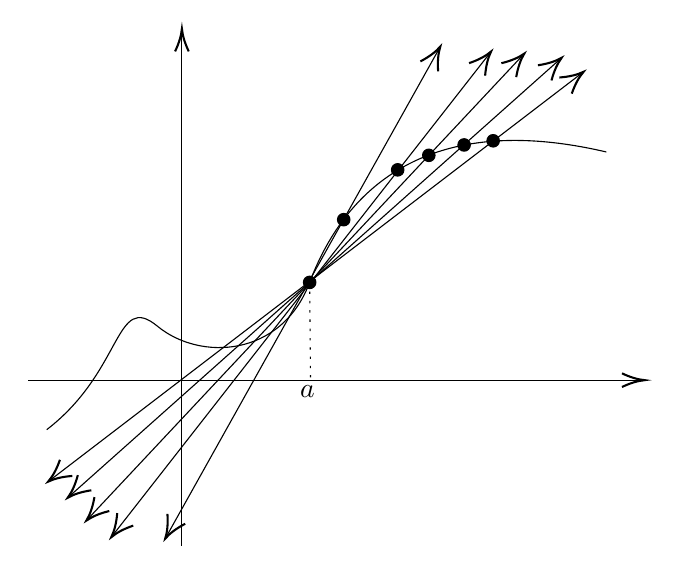
\begin{tikzpicture}[x=0.75pt,y=0.75pt,yscale=-1,xscale=1]
%uncomment if require: \path (0,441); %set diagram left start at 0, and has height of 441

%Straight Lines [id:da16102953695521127]
\draw    (163,221.33) -- (458,221.33) ;
\draw [shift={(460,221.33)}, rotate = 180] [color={rgb, 255:red, 0; green, 0; blue, 0 }  ][line width=0.75]    (10.93,-3.29) .. controls (6.95,-1.4) and (3.31,-0.3) .. (0,0) .. controls (3.31,0.3) and (6.95,1.4) .. (10.93,3.29)   ;
%Straight Lines [id:da9043079513680581]
\draw    (237.04,301) -- (237.04,54) ;
\draw [shift={(237.04,52)}, rotate = 90] [color={rgb, 255:red, 0; green, 0; blue, 0 }  ][line width=0.75]    (10.93,-3.29) .. controls (6.95,-1.4) and (3.31,-0.3) .. (0,0) .. controls (3.31,0.3) and (6.95,1.4) .. (10.93,3.29)   ;
%Curve Lines [id:da7565789477512073]
\draw    (171.9,245.19) .. controls (209.02,216.63) and (204.74,178.41) .. (225.27,195.34) .. controls (245.8,212.28) and (284.99,210.33) .. (298.59,174.22) .. controls (312.18,138.1) and (347.09,89.21) .. (441.52,111.39) ;
%Straight Lines [id:da9796385406474812]
\draw    (428.99,73.97) -- (174.17,269.02) ;
\draw [shift={(172.58,270.23)}, rotate = 322.57] [color={rgb, 255:red, 0; green, 0; blue, 0 }  ][line width=0.75]    (10.93,-4.9) .. controls (6.95,-2.3) and (3.31,-0.67) .. (0,0) .. controls (3.31,0.67) and (6.95,2.3) .. (10.93,4.9)   ;
\draw [shift={(430.57,72.75)}, rotate = 142.57] [color={rgb, 255:red, 0; green, 0; blue, 0 }  ][line width=0.75]    (10.93,-4.9) .. controls (6.95,-2.3) and (3.31,-0.67) .. (0,0) .. controls (3.31,0.67) and (6.95,2.3) .. (10.93,4.9)   ;
%Straight Lines [id:da1158565706067487]
\draw    (384.77,64.58) -- (204.23,295.42) ;
\draw [shift={(203,297)}, rotate = 308.03] [color={rgb, 255:red, 0; green, 0; blue, 0 }  ][line width=0.75]    (10.93,-4.9) .. controls (6.95,-2.3) and (3.31,-0.67) .. (0,0) .. controls (3.31,0.67) and (6.95,2.3) .. (10.93,4.9)   ;
\draw [shift={(386,63)}, rotate = 128.03] [color={rgb, 255:red, 0; green, 0; blue, 0 }  ][line width=0.75]    (10.93,-4.9) .. controls (6.95,-2.3) and (3.31,-0.67) .. (0,0) .. controls (3.31,0.67) and (6.95,2.3) .. (10.93,4.9)   ;
%Straight Lines [id:da7715304094905251]
\draw    (400.63,65.46) -- (192.37,287.54) ;
\draw [shift={(191,289)}, rotate = 313.16] [color={rgb, 255:red, 0; green, 0; blue, 0 }  ][line width=0.75]    (10.93,-4.9) .. controls (6.95,-2.3) and (3.31,-0.67) .. (0,0) .. controls (3.31,0.67) and (6.95,2.3) .. (10.93,4.9)   ;
\draw [shift={(402,64)}, rotate = 133.16] [color={rgb, 255:red, 0; green, 0; blue, 0 }  ][line width=0.75]    (10.93,-4.9) .. controls (6.95,-2.3) and (3.31,-0.67) .. (0,0) .. controls (3.31,0.67) and (6.95,2.3) .. (10.93,4.9)   ;
%Straight Lines [id:da44730990962603356]
\draw    (418.51,67.33) -- (183.49,276.67) ;
\draw [shift={(182,278)}, rotate = 318.31] [color={rgb, 255:red, 0; green, 0; blue, 0 }  ][line width=0.75]    (10.93,-4.9) .. controls (6.95,-2.3) and (3.31,-0.67) .. (0,0) .. controls (3.31,0.67) and (6.95,2.3) .. (10.93,4.9)   ;
\draw [shift={(420,66)}, rotate = 138.31] [color={rgb, 255:red, 0; green, 0; blue, 0 }  ][line width=0.75]    (10.93,-4.9) .. controls (6.95,-2.3) and (3.31,-0.67) .. (0,0) .. controls (3.31,0.67) and (6.95,2.3) .. (10.93,4.9)   ;
%Shape: Circle [id:dp8153494409622872]
\draw  [fill={rgb, 255:red, 0; green, 0; blue, 0 }  ,fill opacity=1 ] (384,106) .. controls (384,104.34) and (385.34,103) .. (387,103) .. controls (388.66,103) and (390,104.34) .. (390,106) .. controls (390,107.66) and (388.66,109) .. (387,109) .. controls (385.34,109) and (384,107.66) .. (384,106) -- cycle ;
%Shape: Circle [id:dp46038093787284295]
\draw  [fill={rgb, 255:red, 0; green, 0; blue, 0 }  ,fill opacity=1 ] (370,108) .. controls (370,106.34) and (371.34,105) .. (373,105) .. controls (374.66,105) and (376,106.34) .. (376,108) .. controls (376,109.66) and (374.66,111) .. (373,111) .. controls (371.34,111) and (370,109.66) .. (370,108) -- cycle ;
%Shape: Circle [id:dp190859565625209]
\draw  [fill={rgb, 255:red, 0; green, 0; blue, 0 }  ,fill opacity=1 ] (353,113) .. controls (353,111.34) and (354.34,110) .. (356,110) .. controls (357.66,110) and (359,111.34) .. (359,113) .. controls (359,114.66) and (357.66,116) .. (356,116) .. controls (354.34,116) and (353,114.66) .. (353,113) -- cycle ;
%Shape: Circle [id:dp3044800797092422]
\draw  [fill={rgb, 255:red, 0; green, 0; blue, 0 }  ,fill opacity=1 ] (338,120) .. controls (338,118.34) and (339.34,117) .. (341,117) .. controls (342.66,117) and (344,118.34) .. (344,120) .. controls (344,121.66) and (342.66,123) .. (341,123) .. controls (339.34,123) and (338,121.66) .. (338,120) -- cycle ;
%Shape: Circle [id:dp7651386739199335]
\draw  [fill={rgb, 255:red, 0; green, 0; blue, 0 }  ,fill opacity=1 ] (295.59,174.22) .. controls (295.59,172.56) and (296.93,171.22) .. (298.59,171.22) .. controls (300.24,171.22) and (301.59,172.56) .. (301.59,174.22) .. controls (301.59,175.87) and (300.24,177.22) .. (298.59,177.22) .. controls (296.93,177.22) and (295.59,175.87) .. (295.59,174.22) -- cycle ;
%Straight Lines [id:da21925282533113744]
\draw  [dash pattern={on 0.84pt off 2.51pt}]  (298.59,174.22) -- (299,221) ;
%Straight Lines [id:da4492754198498514]
\draw    (360.57,62.35) -- (229.98,295.92) ;
\draw [shift={(229,297.67)}, rotate = 299.21] [color={rgb, 255:red, 0; green, 0; blue, 0 }  ][line width=0.75]    (10.93,-4.9) .. controls (6.95,-2.3) and (3.31,-0.67) .. (0,0) .. controls (3.31,0.67) and (6.95,2.3) .. (10.93,4.9)   ;
\draw [shift={(361.54,60.61)}, rotate = 119.21] [color={rgb, 255:red, 0; green, 0; blue, 0 }  ][line width=0.75]    (10.93,-4.9) .. controls (6.95,-2.3) and (3.31,-0.67) .. (0,0) .. controls (3.31,0.67) and (6.95,2.3) .. (10.93,4.9)   ;
%Shape: Circle [id:dp18797969215530874]
\draw  [fill={rgb, 255:red, 0; green, 0; blue, 0 }  ,fill opacity=1 ] (312,144) .. controls (312,142.34) and (313.34,141) .. (315,141) .. controls (316.66,141) and (318,142.34) .. (318,144) .. controls (318,145.66) and (316.66,147) .. (315,147) .. controls (313.34,147) and (312,145.66) .. (312,144) -- cycle ;

% Text Node
\draw (292.79,222.73) node [anchor=north west][inner sep=0.75pt]    {$a$};
% Text Node
\draw (318,60.4) node [anchor=north west][inner sep=0.75pt]    {$\dotsc $};


\end{tikzpicture}

}

\end{multicols}


You'll notice that the tangent line captures some \textit{local information} about $f$ at $a$. In other words, it is a good approximation of $f$ at $a$; that is, $f$ and its tangent line are ``similar'' at $a$. Intuitively, you should think about the tangent line at $a$ to be the line that ``hugs $f$ the best at $a$.''

Note that this definition of the derivative only makes sense if $f$ is defined on an open interval containing $a$. We can view the derivative as a function, and write $[f(x)]'$ or $f'(x)$. The derivative of $f'(x)$ is called the \textbf{second derivative} and is denoted $f''(x)$. In general, the $n$th derivative $f^{(n)}(x)$ is defined to be the derivative of $f^{(n-1)}(x)$.

\subsection{The Two Part ``Program'' for Finding Derivatives}

So now we have a goal: find derivatives of functions. The problem is that the limit definition is difficult to use (that pesky $h\to 0$ in the denominator). So instead, we will do the following two steps (let $a$ be a real number and $f$ and $g$ be functions):
\begin{enumerate}
\item rules to break functions up and reassemble

\begin{center}
\def\arraystretch{1.5}
\begin{tabular}{@{}ll@{}}
\toprule[0.4mm]
\textbf{The Scalar Multiple Rule} & $[af]' = af'$. \\
\textbf{The Sum Rule} & $[f + g]' = f' + g'$ \\
\textbf{The Product Rule} & $[fg]' = f'g + fg'$ \\
\textbf{The Quotient Rule} & $\left[\frac{f}{g}\right]' = \frac{f'g - fg'}{g^2}$ \\
\textbf{The Chain Rule} & $[f(g(x))]' = f'(g(x))g'(x)$ \\
\textbf{The Inverse Rule} & $[f^{-1}(x)]' = \frac{1}{f'(f^{-1}(x))}$ \\
\bottomrule[0.4mm]
\end{tabular}
\end{center}

\item find derivatives of ``basic'' functions:

\end{enumerate}


\begin{center}
\def\arraystretch{1.5}
\begin{tabular}{@{}ll@{}}
\toprule[0.4mm]
\textbf{The Constant Rule}     & $[a]' = 0$ \\
\textbf{The Power Rule}        & $[x^a]' = ax^{a-1}$ \\
\textbf{Trig Rules}  & $[\sin(x)]' = \cos(x)$ and $[\cos(x)]' = -\sin(x)$ \\
\textbf{Exponential Rules} & $[a^x]' = \ln(a)a^x$ \\
\textbf{Logarithmic Rules} & $[\log_a(x)]' = \frac{1}{x\ln(a)}$ \\
\bottomrule[0.4mm]
\end{tabular}
\end{center}


Most of the time, you will be able to find the derivatives using a combination of these rules. For instance, the derivatives of the other 4 trig functions can be found using the quotient rule and the derivatives of $\sin$ and $\cos$:
$$[\tan(x)]' = \sec^2(x)
\quad\quad\quad\quad\quad
[\sec(x)]' = \sec(x)\tan(x)$$

$$[\cot(x)]' = -\csc^2(x)
\quad\quad\quad\quad\quad
[\csc(x)]' = -\csc(x)\cot(x)$$
\mar{Try to find the pattern with these four derivatives.}


\subsection{Implicit Differentiation}

We'll refer to the set of points that satisfy an equation of two variables as a \textbf{curve in the plane}. Some examples you might have seen before are circles and ellipses. The circle with center $(h,k)$ and radius $r$ is the set of points $(x,y)$ in the plane that satisfy the equation
$$(x-h)^2+(y-k)^2=r^2.$$
\mar{Look up the similar equation for an ellipse and write it down here.}

In general, curves are not functions (they might not pass the vertical line test), but they can still have tangent lines, so we should be able to describe their slope at a point. We do this by ``zooming in'' on a point of the curve, and forgetting about the other parts of the curve. Now (locally), it looks like a function, so we can treat the $y$ variable as a function of $x$. This process is called ``implicit'' differentiation, and consists of two steps:
\begin{enumerate}
\item differentiate both sides of the equation (keeping in mind that since $y$ is a function of $x$, the derivative of $f(y)$ is $f'(y)\cdot y'$ by the chain rule).
\item solve for $y'$.
\end{enumerate}

Other notation is sometimes used: if $y=f(x)$, $\frac{dy}{dx}=\frac{d}{dx}[f(x)]$ is the derivative of $f$, and $\frac{d^ny}{dx^n}=\frac{d^n}{dx^n}[f(x)]$ is the $n$th derivative of $f$.

When you solve for $y'$, it is possible that the expression will consist of both $y$ and $x$ variables. That is because the formula for $y'$ is not a function of just $x$, it is a function of both $x$ and $y$!

Let's do an example:
\begin{itemize}
\item The curve of points satisfying the equation $y^{3}=x^{2}-xy-1$ is not a function, since it does not pass the vertical line test: both $(-1,-1)$ and $(-1,1)$ are solutions. However, we can still find the derivative at each point on this curve! Start by taking the ($x$) derivative of both sides.

On the left, the $x$ derivative of $y^3$ is $3y^2y'$, by the power rule (and the chain rule). The derivative of $x^2$ is $2x$, the derivative of $xy$ is $y+xy'$ by the product rule (and chain rule), and the derivative of $1$ is 0, of course. Comparing the derivatives of each side of the equation, we get
$$3y^2y'=2x-(y+xy'),$$
so solving for $y'$, we have
$$y'=\frac{2x-y}{3y^2+x}.$$
At $(-1,1)$, $y'=\frac{-3}{2}$, and at $(-1,-1)$, $y'=\frac{-1}{2}$. The tangent line to the curve at the point $(-1,1)$ is $y=\frac{-3}{2}(x+1)+1$

\end{itemize}

\subsection{Parametric Curves}

A \textbf{parametric curve} is a curve defined by two coordinate functions $(x(t), y(t))$. You should think of $(x,y)$ as the position of some particle and the particle's coordinates $x(t)$ and $y(t)$ are functions of time.

To find the slope (AKA derivative) of a parametric curve at time $t$, simply compute
$$\frac{dy}{dx}=\frac{y'(t)}{x'(t)}.$$
An example:
\begin{itemize}
    \item The derivative of the curve $(x,y)=(\sin(t), t^2)$ is
    $$\frac{y'(t)}{x'(t)}=\frac{2t}{\cos(t)}.$$
    The equation of the tangent line at $t=\pi$ is $y=\pi^2+\frac{2\pi}{-1}(x-0).$
\end{itemize}

\subsection{Logarithmic Differentiation}

Sometimes you will be faced with a function whose formula includes an expression involving $x$ raised to a power that also involves $x$. Finding the derivative of such a function has a specific procedure:
\begin{strat}[Logarithmic Differentiation]
Suppose $y=f(x)^{g(x)}$ and we want to find $y'$. First apply the $\ln$ function to both sides of the equation and use the log property $\ln(a^b)=b\ln(a)$:
$$\ln(y)=\ln(f(x)^{g(x)})=g(x)\ln(f(x)).$$
Then implicit differentiation yields
$$\frac{1}{y}y'=g'(x)\ln(f(x))+g(x)\frac{f'(x)}{f(x)},$$
and solving for $y'$ and substituting $y=f(x)^{g(x)}$ we get
$$y'=f(x)^{g(x)}\left(g'(x)\ln(f(x))+g(x)\frac{f'(x)}{f(x)}\right).$$
\end{strat}

Here are some examples:
\begin{itemize}
\item $[x^x]'=x^x(\ln(x)+1)=\ln(x^{x^x})+x^x$. (Here $f(x)=g(x)=x$).
\item $[\sin(x)^x]'=\sin(x)^x(\ln(\sin(x))+x\cot(x))$. (Here $f(x)=\sin(x)$ and $g(x)=x$). \mar{Work these examples out.}
\end{itemize}

I don't recommend that you memorize the formula for $[f(x)^{g(x)}]'$. Instead, remember the procedure and re-create when you need it.


\subsection{Using The Inverse Rule}

When we want to find the derivative of an inverse of a function $f$, the inverse rule tells us that
$$[f^{-1}(x)]'=\frac{1}{f'(f^{-1}(x))},$$
but how is this helpful? It is actually very easy to see why this rule is true:
\begin{align*}
         & f(f^{-1}(x)) = x & & \text{(definition of inverse)}\\
\implies & f'(f^{-1}(x))[f^{-1}(x)]'=1 & &\text{(chain rule)}\\
\implies & [f^{-1}(x)]' = \frac{1}{f'(y)} & & \text{(solve for $[f^{-1}(x)]'$)}\\
\implies & [f^{-1}(x)]' =\frac{1}{f'(f^{-1}(x))} & & \text{(substitute)}
\end{align*}

Let's use this rule to find the derivative of inverse trig functions:
\begin{itemize}
\item The rule says that $[\sin^{-1}(x)]'=\frac{1}{\cos(\sin^{-1}(x))}$, but we should be able to simplify this expression using the unit circle.
\begin{figure}[h!]
\centering
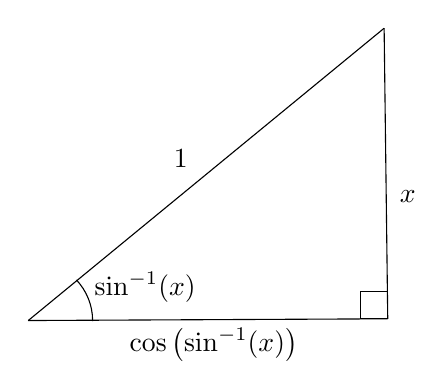
\begin{tikzpicture}[x=0.75pt,y=0.75pt,yscale=-1,xscale=1]
%uncomment if require: \path (0,479); %set diagram left start at 0, and has height of 479

%Straight Lines [id:da021711983663396772]
\draw    (216.29,266.83) -- (389.5,266) ;
%Straight Lines [id:da1995895124000051]
\draw    (387.76,126) -- (216.29,266.83) ;
%Shape: Arc [id:dp31180800912218465]
\draw  [draw opacity=0] (239.51,247.26) .. controls (244.36,252.47) and (247.3,259.32) .. (247.3,266.83) .. controls (247.3,266.94) and (247.3,267.05) .. (247.3,267.16) -- (216.29,266.83) -- cycle ; \draw   (239.51,247.26) .. controls (244.36,252.47) and (247.3,259.32) .. (247.3,266.83) .. controls (247.3,266.94) and (247.3,267.05) .. (247.3,267.16) ;
%Straight Lines [id:da12311387270862384]
\draw    (387.76,126) -- (389.5,266) ;
%Shape: Square [id:dp5026691075905794]
\draw   (376.5,253) -- (389.5,253) -- (389.5,266) -- (376.5,266) -- cycle ;

% Text Node
\draw (247,242) node [anchor=north west][inner sep=0.75pt]    {$\sin^{-1}( x)$};
% Text Node
\draw (263.9,269) node [anchor=north west][inner sep=0.75pt]   [align=left] {$\displaystyle \cos\left(\sin^{-1}(x)\right)$};
% Text Node
\draw (285.15,183.17) node [anchor=north west][inner sep=0.75pt]   [align=left] {$\displaystyle 1$};
% Text Node
\draw (394.13,203) node [anchor=north west][inner sep=0.75pt]   [align=left] {$\displaystyle x$};


\end{tikzpicture}
\end{figure}

\mar{Argue this using the Pythagorean identitiy ($\sin^2\theta+\cos^2\theta = 1$) instead.}

if a (non-right) angle of a right triangle (with hypotenuse 1) is $\sin^{-1}(x)$, the leg opposite $\sin^{-1}(x)$ has length $x$. Then $\cos(\sin^{-1}(x))$ is the length of the other leg of the triangle, so $\cos(\sin^{-1}(x))=\sqrt{1-x^2}$ by the Pythagorean theorem. Therefore,
$$[\sin^{-1}(x)]'=\frac{1}{\cos(\sin^{-1}(x))}=\frac{1}{\sqrt{1-x^2}}.$$\item The derivatives of the other inverse trig functions are
\mar{Figure these equations out by yourself using the same method as for $\sin^{-1}$. Hint: refer to Figure \ref{6trig}}
\begin{align*}
[\cos^{-1}(x)]' & =\frac{-1}{\sqrt{1-x^2}} \\
[\csc^{-1}(x)]' & =\frac{-1}{|x|\sqrt{x^2-1}} \\
[\sec^{-1}(x)]' & =\frac{1}{|x|\sqrt{x^2-1}} \\
[\tan^{-1}(x)]' & =\frac{1}{1+x^2} \\
[\cot^{-1}(x)]' & =\frac{-1}{1+x^2}
\end{align*}
\end{itemize}

% \subsection{Summary}

% \begin{strat}[Finding the Derivative of a Function]
% \begin{enumerate}
% \item
% \end{enumerate}

% \end{strat}


